%% LyX 2.2.3 created this file.  For more info, see http://www.lyx.org/.
%% Do not edit unless you really know what you are doing.
\documentclass[oneside,english]{extbook}
\usepackage{lmodern}
\renewcommand{\sfdefault}{lmss}
\renewcommand{\ttdefault}{lmtt}
\usepackage[T1]{fontenc}
\usepackage[latin9]{inputenc}
\usepackage{geometry}
\geometry{verbose,tmargin=25mm,bmargin=25mm,lmargin=25mm,rmargin=25mm}
\setcounter{secnumdepth}{3}
\setcounter{tocdepth}{3}
\setlength{\parindent}{0bp}
\usepackage{babel}
\usepackage{float}
\usepackage{graphicx}
\usepackage{setspace}
\onehalfspacing
\usepackage[unicode=true,pdfusetitle,
 bookmarks=true,bookmarksnumbered=false,bookmarksopen=false,
 breaklinks=false,pdfborder={0 0 1},backref=false,colorlinks=false]
 {hyperref}

\makeatletter
%%%%%%%%%%%%%%%%%%%%%%%%%%%%%% User specified LaTeX commands.
\usepackage{amssymb}
\usepackage{color}
\usepackage{listings}
\definecolor{hellgelb}{rgb}{1,1,0.85}
\definecolor{colKeys}{rgb}{0,0,1}
\definecolor{colIdentifier}{rgb}{0,0,0}
\definecolor{colComments}{rgb}{1,0,0}
\definecolor{colString}{rgb}{0,0.5,0}
\lstset{
      language=Matlab,
      float=hbp,
      basicstyle=\footnotesize\ttfamily,
      identifierstyle=\color{colIdentifier},
      keywordstyle=\color{colKeys},
      stringstyle=\color{colString},
      commentstyle=\itshape\color{colComments},
      columns=fixed,
      tabsize=4,
      frame=single,
      framerule=1pt,
      extendedchars=true,
      showspaces=false,
      showstringspaces=false,
      numbers=left,
      numberstyle=\tiny\ttfamily,
      numbersep=1em,
      breaklines=true,
      breakindent=10pt,
      backgroundcolor=\color{hellgelb},
      breakautoindent=true,
      captionpos=t,
      xleftmargin=1em,
      xrightmargin=\fboxsep
}
\usepackage{lscape}
\usepackage{amsmath}
\usepackage{mathtools}
\usepackage{pifont}
\usepackage{color}
\usepackage{pdfpages}
\usepackage{accents}
\delimitershortfall=-1pt
\let\Right\right
\let\Left\left
\makeatletter
\def\right#1{\Right#1\@ifnextchar){\!\right}{}}
\def\left#1{\Left#1\@ifnextchar({\!\left}{}}
\makeatother

\setcounter{MaxMatrixCols}{20}

\makeatother

\begin{document}
\pagenumbering{gobble}

\includepdf{../FIGURES/fig02.pdf}

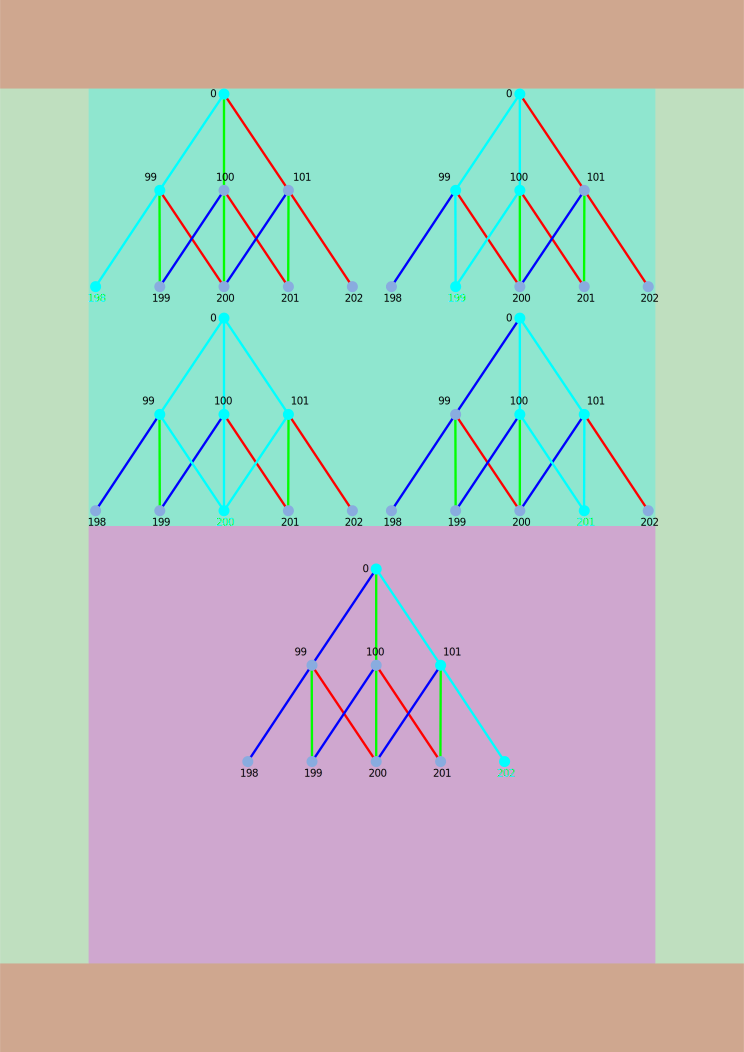
\includepdf{../FIGURES/fig04.pdf}

\includepdf{../FIGURES/fig06.pdf}

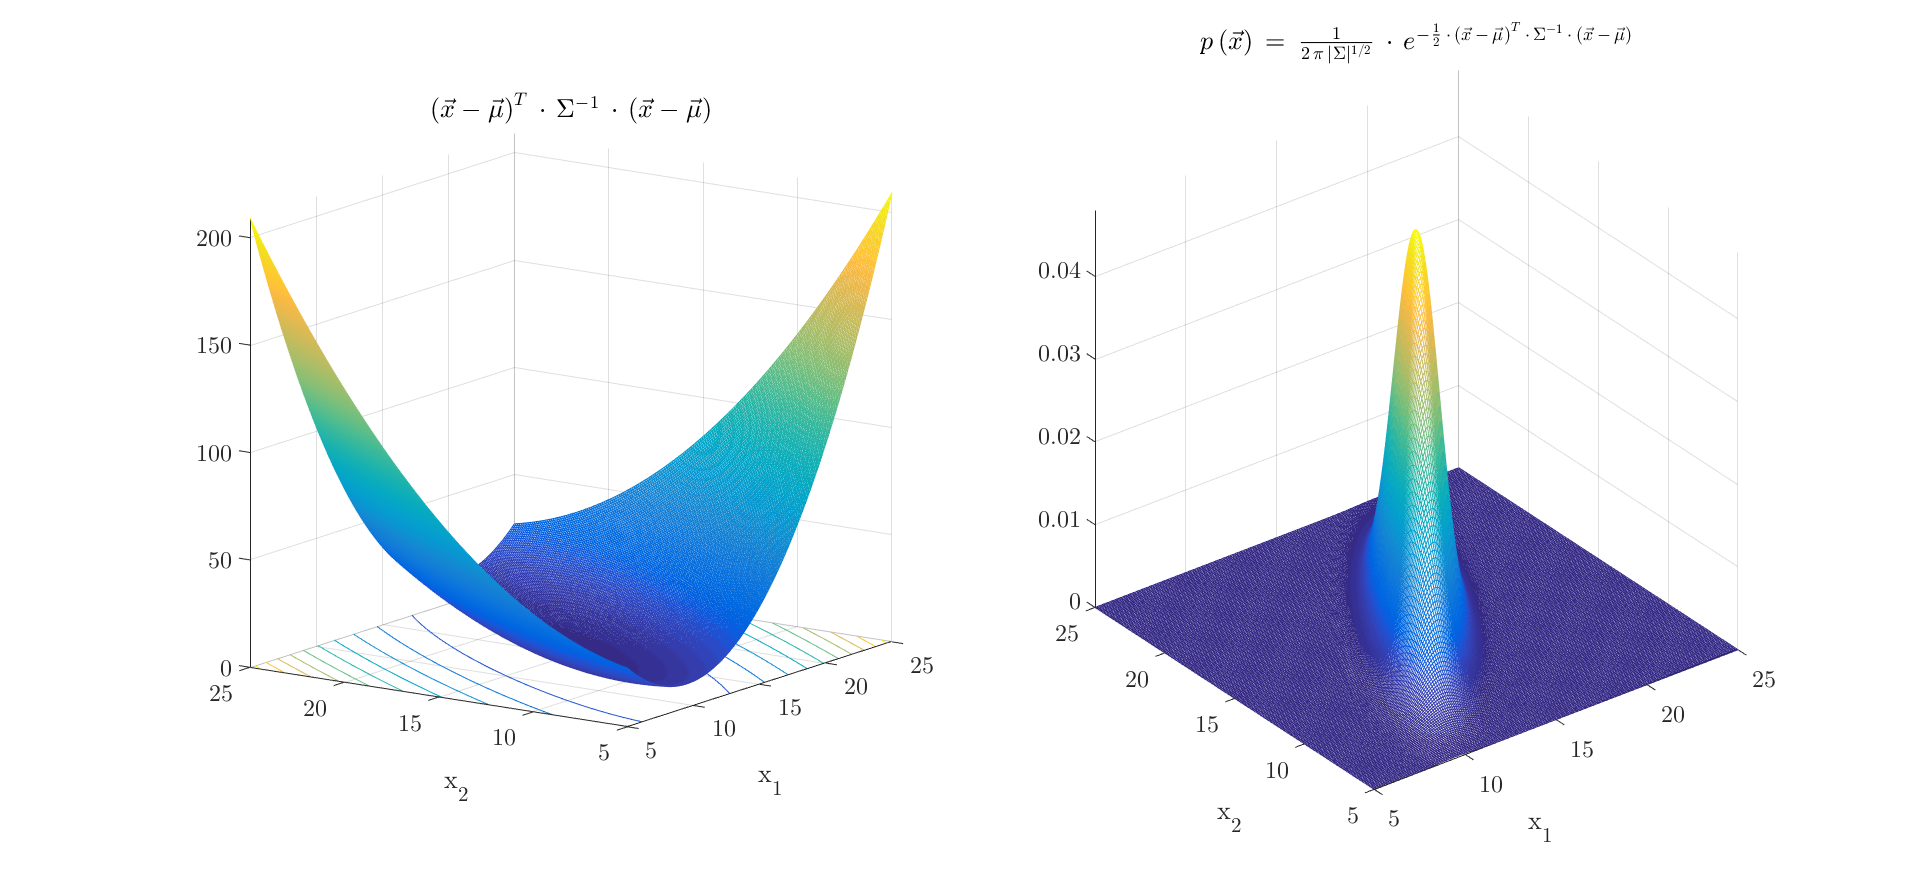
\includepdf{../FIGURES/fig08.pdf}

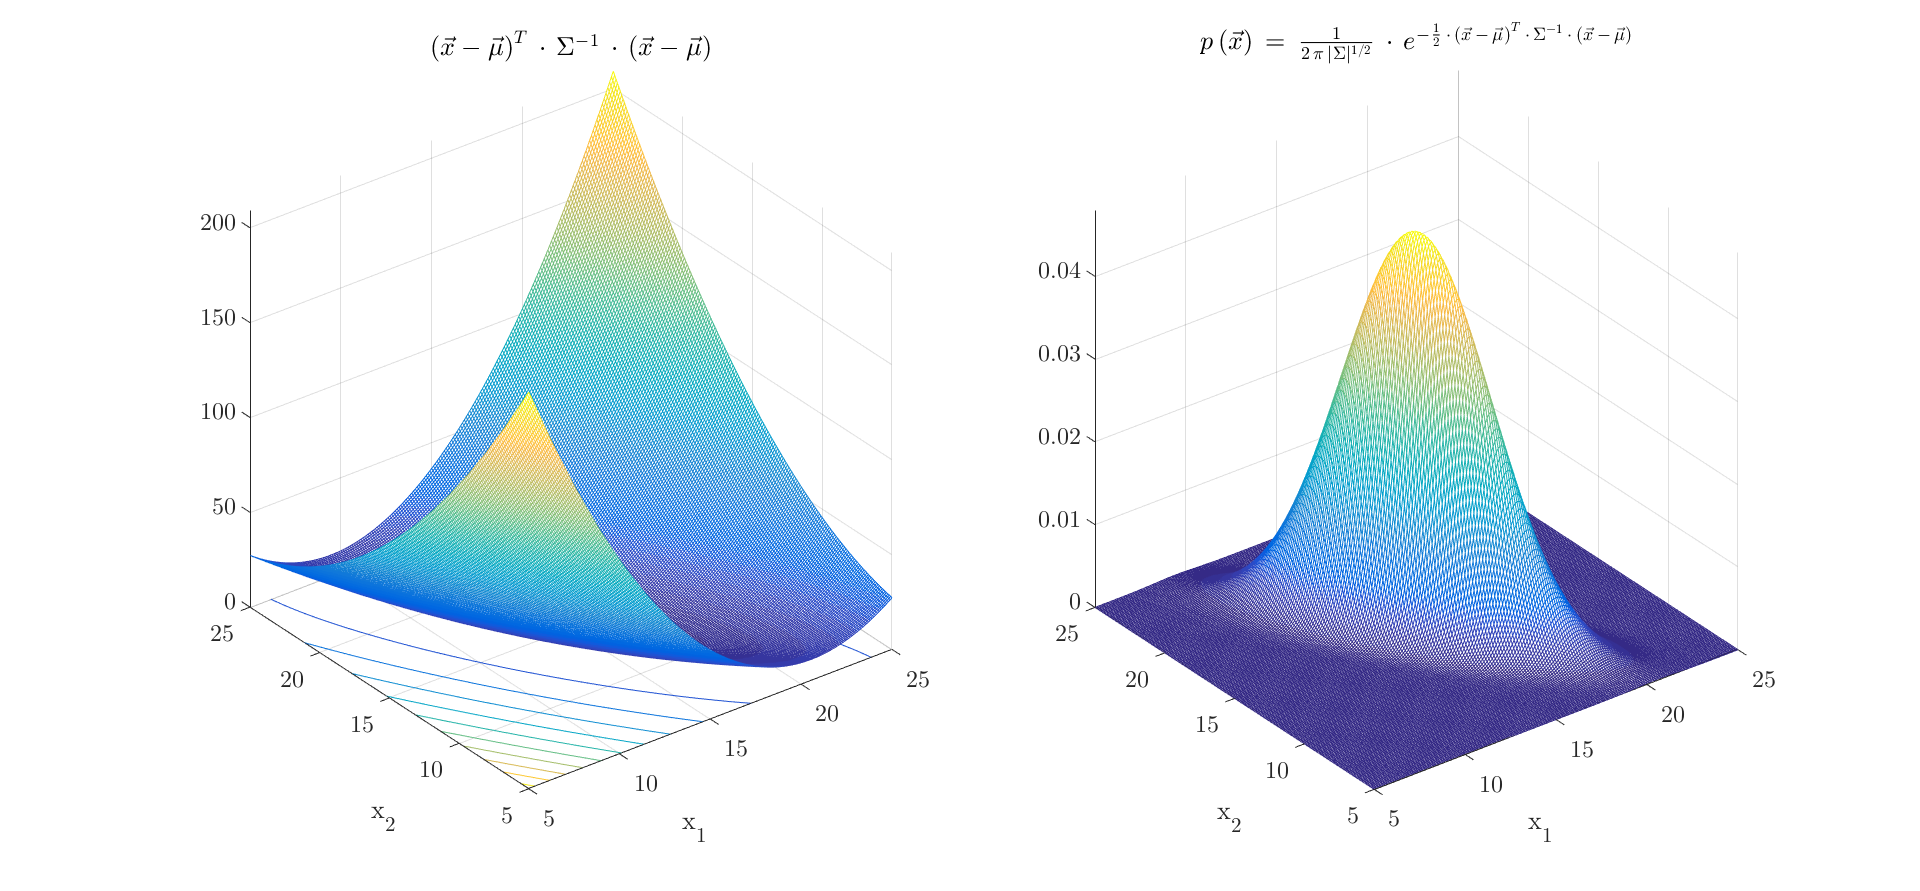
\includepdf{../FIGURES/fig10.pdf}

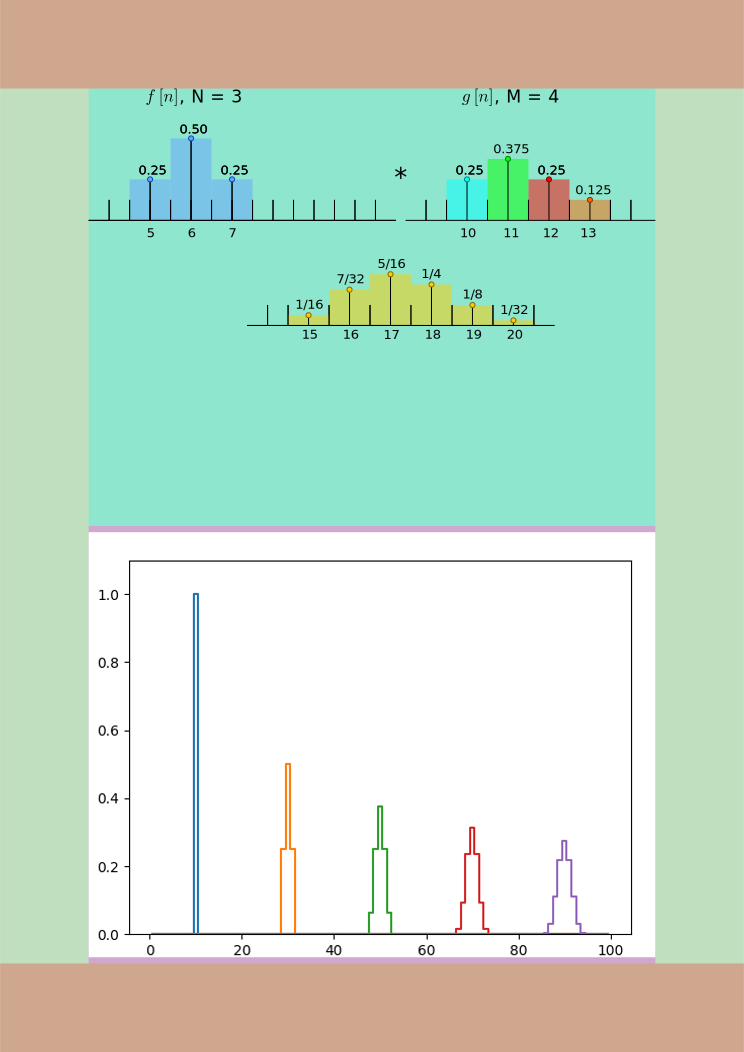
\includepdf{../FIGURES/fig12.pdf}

\includepdf{../FIGURES/fig14.pdf}

\includepdf{../FIGURES/fig16.pdf}

\begin{figure}[H]
\centering\includegraphics[scale=0.9]{../FIGURES/fig17}
\end{figure}

We want to paint the nodes for where the Dijkstra algorithm passes
in different tonalities of the same color according to its cost. The
first idea is to use two matrices, one for visited nodes and one for
the cost of each node. But, we can achieve the same behavior using
only one matrix, the visited node matrix. Instead of storing 1 or
0 in the visited node matrix, we store the cost of the node. So, a
cost$\,>\,0$ means that a node has already been visited. We have
to do one trick, then. The starting node has to have another cost
different from 0, because a cost of 0 means not visited yet. So, for
the starting node we use the cost 0.001. This value is small enough
to show that the starting point has been visited and also it will
be the smallest cost in the graph.

\begin{figure}[H]
\centering\includegraphics[scale=0.8]{../FIGURES/fig18}
\end{figure}

\includepdf{../FIGURES/fig20.pdf}

\includepdf{../FIGURES/fig22.pdf}

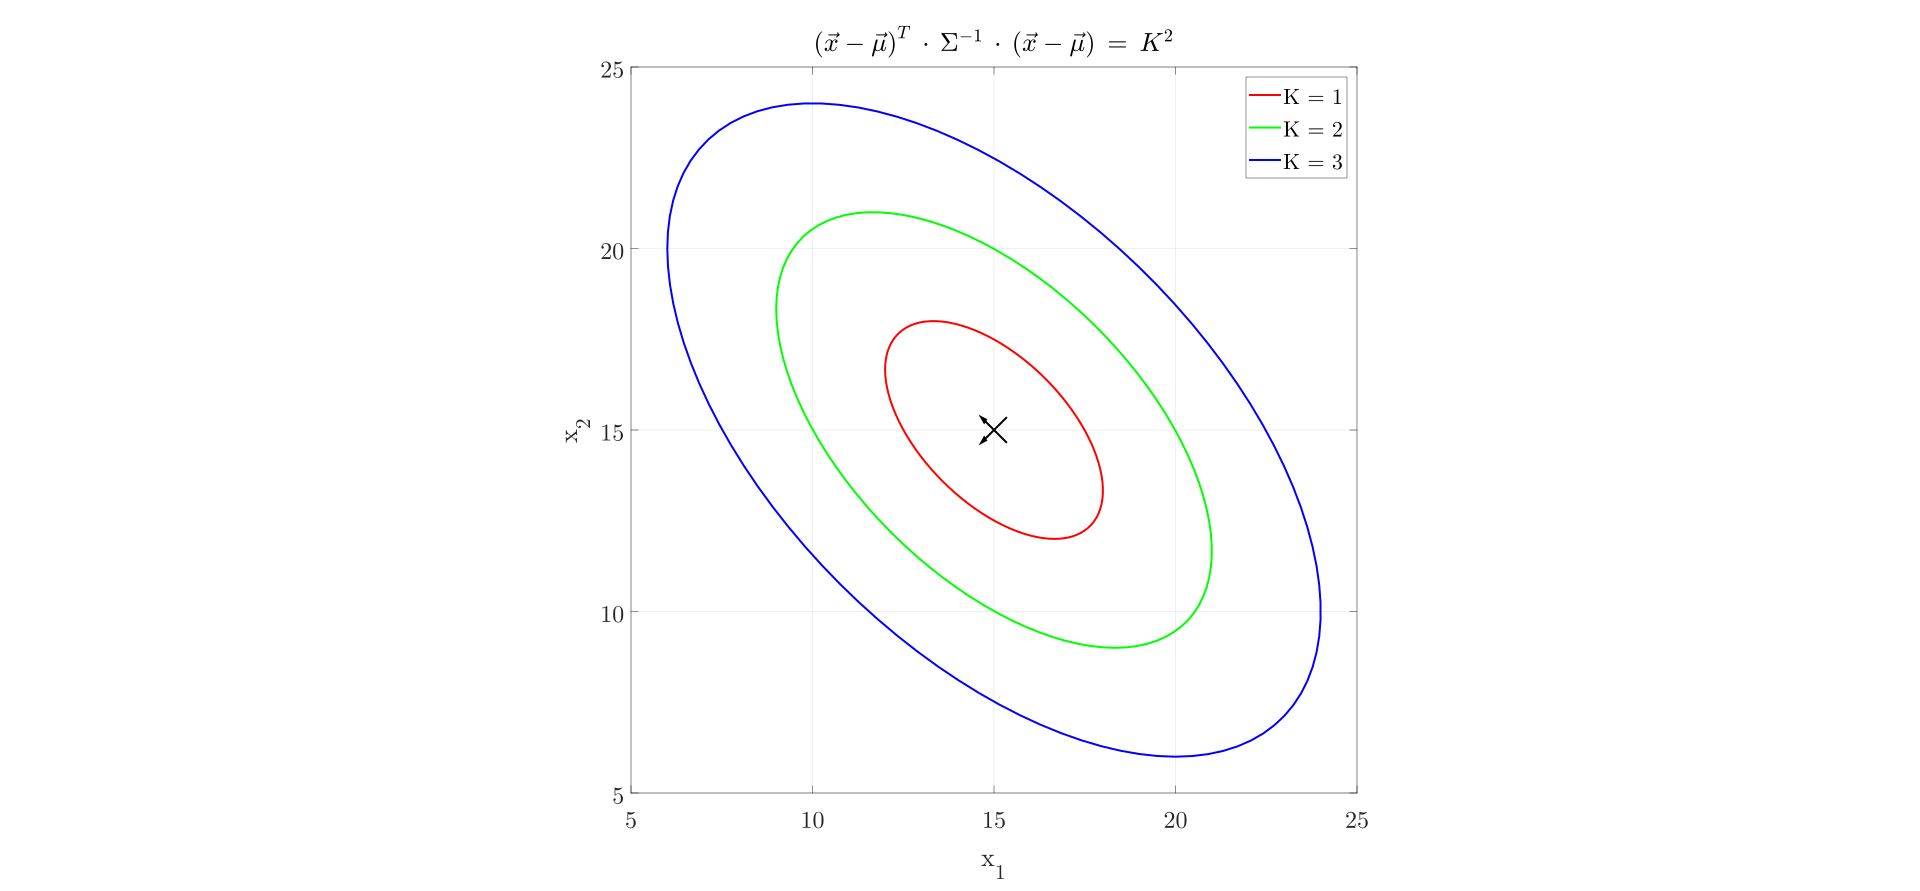
\includepdf{../FIGURES/fig24.pdf}

\includepdf{../FIGURES/fig26.pdf}
\end{document}
